\documentclass[a4paper,10pt,pagesize,titlepage]{scrbook}

% \usepackage[utf8x]{inputenc}
\usepackage[ngerman]{babel}
\usepackage{caption}
\usepackage{fontenc}
\usepackage{graphicx}
\usepackage[utf8]{inputenc}
\usepackage[T1]{fontenc}
% \usepackage{microtype}
\usepackage{bbm}
\usepackage{keystroke}
\usepackage{amsmath}
\usepackage{colortbl}
\usepackage{color}
\usepackage{array}
\usepackage{textcomp}
\usepackage{makeidx}
\usepackage{float}
\usepackage{rotating}
\usepackage{longtable}
\usepackage{cite}
\usepackage{listings}
% \usepackage{capt-of}
\usepackage{booktabs}
\usepackage{url}
\usepackage{hyperref}
\def\UrlBreaks{%
	\do\/%
	\do\a\do\b\do\c\do\d\do\e\do\f\do\g\do\h\do\i\do\j\do\k\do\l%
	\do\m\do\n\do\o\do\p\do\q\do\r\do\s\do\t\do\u\do\v\do\w\do\x\do\y\do\z%
	\do\A\do\B\do\C\do\D\do\E\do\F\do\G\do\H\do\I\do\J\do\K\do\L%
	\do\M\do\N\do\O\do\P\do\Q\do\R\do\S\do\T\do\U\do\V\do\W\do\X\do\Y\do\Z%
	\do0\do1\do2\do3\do4\do5\do6\do7\do8\do9\do=\do/\do.\do:%
	\do\*\do\-\do\~\do\'\do\"\do\-}


\definecolor{lightturquoise}{rgb}{0.9,0.8,0.7}
\definecolor{honeydew}{rgb}{0.9,0.6,0.8}
\definecolor{khaki}{rgb}{0.8,0.8,0.95}
\definecolor{tablegrey}{rgb}{0.800,0.800,0.800}
\definecolor{tablelightgrey}{rgb}{0.900,0.900,0.900}
\definecolor{hellgrau}{rgb}{0.95,0.95,0.95}
\newcommand{\teaser}[2]%
{{\list{}{\rightmargin0pt\leftmargin30pt}\item\relax\textit{#1}\endlist%
}}

\newcommand{\menue}{\textbf}
\newcommand{\schaltflaeche}{\textbf}
\newcommand{\befehl}{\textbf}
\newcommand{\kontextmenue}{\textbf}
\newcommand{\dialog}{\textbf}
\newcommand{\symbolleiste}{\textbf}
\newcommand{\register}{textbf}

\lstset{literate={ä}{{\"a}}1	
	}
\lstset{literate={ö}{{\"o}}1	
}
\lstset{literate={ü}{{\"u}}1	
}

\author{Andreas Mantke}
\title{Erweiterungen für LibreOffice erstellen}
\date{\today}

\makeindex

\begin{document}

% Festlegung Art der Zitierung - Havardmethode: Abkuerzung Autor + Jahr
\bibliographystyle{plain} 


\maketitle
 \setcounter{tocdepth}{10}


\begin{flushleft}
	
	\textit{Erweiterungen für LibreOffice erstellen}
	
	© Andreas Mantke 
	
	
	\noindent This work is licensed under a Creative Commons Attribution-NonCommercial 4.0 International License. Dieses Werk ist lizenziert unter der Creative Commons Attribution-NonCommercial 4.0 International License.
	https://creativecommons.org/licenses/by-nc/4.0/
	https://creativecommons.org/licenses/by-nc/4.0/legalcode
\end{flushleft}


\tableofcontents
\listoffigures

\chapter*{Vorwort}

Für das Entwickeln von LibreOffice finden sich Informationen auf verschiedenen Ressourcen. Zum Teil muss ersatzweise auf - nicht immer noch aktuelle - Informationen zu OpenOffice.org zurückgegriffen werden. Das Ziel dieses Dokumentes ist es, möglichst detaillierte Informationen zur eigenständigen Entwicklung von neuen LibreOffice Extensions zu geben. Die Darstellung soll dabei anhand von Beispielen erfolgen. Diese werden die unterschiedlichen Bereiche beleuchten, mit denen sich weitere oder besondere Inhalte oder neue bzw. erweiterte Funktionen zu LibreOffice hinzugefügt werden können. Es geht also sowohl um beispielsweise das Hinzufügen von eigenen Themen zur sogenannten Gallery wie auch um weitere Funktionalität unter Verwenden von Programmiersprachen, wie z.B. Python. Für die letztere Programmiersprache bringt LibreOffice bereits eine Umgebung von Python 3 mit.

Das Dokument ist eine Arbeit im Fluss und wird nach und nach um weitere Kapitel ergänzt werden. Es ist aktuell nur in deutscher Sprache verfügbar. Eine Lokalisation in anderen Sprachen ist aber für die Zukunft eine Option.

\chapter{Arten von Erweiterungen}
Für LibreOffice können Sie Extensions (Erweiterungen) erstellen, die mit verschiedenen Programmiersprachen arbeiten. Es sind die folgenden Sprachen verfügbar:
\begin{itemize}
	\item C++
	\item Python
	\item Java
	\item JavaScript
	\item LibreOffice Basic
\end{itemize}
Außerdem können Sie mit Extensions auch Konfigurationsdateien für LibreOffice für Ihre Benutzer beispielsweise im Rahmen einer automatischen Installation ausrollen. Mit Extensions können Sie auch eine neue Gallery (Zusammenstellung von Grafiken), weitere Paletten, Autotexte oder Assistenten für LibreOffice bereit stellen.

Alle Erweiterungen von LibreOffice werden in einer komprimierten Container-Datei mit der Dateiendung .oxt gepackt. Sie können, sofern Sie unter einer freien Software-Lizenz stehen, über die Seite https://extensions.libreoffice.org veröffentlicht und geteilt bzw. zum Download angeboten werden.

\chapter{Der Container OXT und sein Inhalt}\label{oxtcontainerinhalt}
Innerhalb des komprimierten Datei-Containers OXT befinden sich mehrere Dateien und es ist regelmäßig auch eine spezielle Struktur angelegt. Diese Struktur und der Inhalt der einzelnen Dateien des Containers sollen nun anhand eines konkreten Beispiels erläutert werden. Diese Beispielextension soll den Namen myfirstextension.oxt führen. Wir erstellen dazu zunächst ein Verzeichnis mit dem Namen myfirstextension. In diesem erzeugen wir dann die Textdatei description.xml, die wir im folgenden Abschnitt bearbeiten.
\section{Die Datei description.xml}
Wir öffnen nun die zuvor erstellte Datei description.xml mit einem Texteditor. Diese Datei wird die wesentlichen Verwaltungsinformationen der Extension enthalten.
Sie startet mit einer XML-Deklaration einschließlich Encoding:
\begin{lstlisting}
<?xml version="1.0" encoding="UTF-8"?>
\end{lstlisting}
Danach folgt das Description-Tag, das mit einer Definition versehen ist und als Root alle beschreibenden Elemente einschließt:
\begin{lstlisting}
<description
     xmlns="http://openoffice.org/extensions/description/2006"
     xmlns:xlink="http://www.w3.org/1999/xlink">
</description>
\end{lstlisting}
Bereits mit diesem rudimentären Inhalt könnte die Extension als komprimierter OXT-Container (Zip-Container) vom LibreOffice Extension-Manager geladen werden, allerdings fehlen für den Anwender noch die wesentlichen Grundinformationen und die Extension hat auch noch keine Funktionalität.

Sofern sich bei der Vorgabe der Deklaration des Namespace im <description>-Tag ein Fehler (z.B. ein Tippfehler) eingeschlichen hat, erhalten Sie eventuell beim Versuch der Installation der Extension eine Fehlermeldung wie im Bildschirmfoto unten.
\begin{center}
	\captionsetup{type=figure}
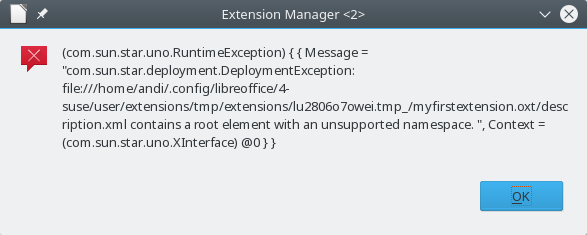
\includegraphics[width=0.7\linewidth]{pics/error_wrong_namedeclaration}
\captionof{figure}{Fehlermeldung wegen fehlerhafter Namespace-Deklaration}
\label{fig:error_wrong_namedeclaration}
\end{center}


\paragraph*{Identifier}$~~$\\

Als erste Ergänzung fügen wir in das Description-Tag einen sogenannten Identifier ein. Dies ist eine eindeutige Bezeichnung der Extension für den LibreOffice Extensionmanager. Es ist möglich, dass zwei inhaltlich bzw. auf Dateiebene identische Extensions vom Extensionmanager geladen werden, sofern sie unterschiedliche Identifier haben, nicht aber anders herum. Deshalb ist es wichtig, dass sie einen Identifier wählen, auf den nur Sie Zugriff haben bzw. der regelmäßig nur von Ihnen in dieser Form gewählt werden wird.

Der Identifier spielt dabei auch bei einem eventuell vorgesehenen Online-Update der Extension später eine wesentliche Rolle. Für unser Beispiel verwenden wir:
\begin{lstlisting}
<identifier value="org.mycompany.myfirstextension" />
\end{lstlisting}

\paragraph*{Version}$~~$\\

Als nächstes fügen wir die Angabe der Versionsnummer (Release-Nummer) der Extension in das Description-Tag als neues Tag ein:
\begin{lstlisting}
<version value="0.1" />
\end{lstlisting}
Als Werte (Value) kommen hier positive Zahlen in Betracht, die eine Versionsnummer der Extension darstellen können. Die Versions-Nummer kann aus lediglich einer positiven Ziffer (größer Null) oder einer Kolonne von mehreren durch Punkt getrennten Ziffern bestehen, z.B. 0.1.3. Das Benennungsschema sollte dabei den üblichen Geflogenheiten folgen. Die erste Ziffer bezeichnet insoweit Major-(Haupt-)Releases (mit eventueller Inkompatibilität zu bisherigen Haupt-Releases). Die zweite Ziffer steht für Änderungen im Sinne von Minor-Releases (mit kompatiblen Änderungen), während die dritte Ziffer Micro-Releases anzeigt (mit beispielsweise Fehlerbereinigungen).

\paragraph*{Plattform}$~~$\\

Eine LibreOffice Extension kann sowohl für alle Plattformen von LibreOffice lauffähig sein, als auch lediglich für einzelne. Dies wird über das Platform-Tag gesteuert. Wir gehen davon aus, dass die Extension für alle Plattformen geeignet ist und fügen daher folgendes Zeile ein:
\begin{lstlisting}
<platform value="all" />
\end{lstlisting}
Der Wert ("value") kann entweder eine oder mehrere Plattformen mit Komma getrennt enthalten. Beispielsweise in folgender Form:
\begin{lstlisting}
<platform value="windows_x86, linux_x86_64, linux_x86" /> 
\end{lstlisting} 
Die Extension kann nur installiert werden, wenn eine der angegebenen Plattformen dem laufenden Betriebssystem entspricht. Falls als Wert keine Plattform angegeben wird, kann die Extension unter keinem laufenden Betriebssystem installiert werden.
\begin{lstlisting}
<platform value=" " />
\end{lstlisting}
Der Extensionmanager von LibreOffice kann hier keine Plattform (Betriebssystem) ausfindig machen, auf dem die Extension lauffähig ist, und bricht daher die Installation ab.

Die folgende Tabelle listet alle möglichen Plattformen auf, die als Wert verwendet werden können, unabhängig davon, ob sie von LibreOffice unterstützt werden.\linebreak


\begin{tabular}{ |p{3cm}|p{9cm} | }
	
	\multicolumn{2}{l}{\textbf{Platform Token (Plattform-Schlüssel)}}\\
	\toprule
	\rowcolor{hellgrau}
	Token (Schlüssel)& Beschreibung\\
	\hline
	all   & Umfasst alle Plattformen\\
	\hline
    \verb|freebsd_x86|& FreeBSD Betriebssystem auf X86-Plattform\\
    \hline
    \verb|freebsd_x86_64|& FreeBSD Betriebssystem auf 64bit-Plattform\\
    \hline
    \verb|linux_arm_eabi|& (Aktuell nicht unterstützt) Linux Betriebssystem auf einer ARM-CPU unter Verwenden von "EABI"\\
    \hline
    \verb|linux_arm_oabi|& (Aktuell nicht unterstützt) Linux Betriebssystem auf einer ARM-CPU unter Verwenden von "OABI"\\
    \hline
    \verb|linux_ia64| &	Linux Betriebssystem auf einer ia64 CPU\\
    \hline
    \verb|linux_mips_eb| &	(Aktuell nicht unterstützt) Linux Betriebssystem auf einer MIPS CPU unter verwenden von 'EB' ABI\\
    \hline
    \verb|linux_mips_el| &	(Aktuell nicht unterstützt) Linux Betriebssystem auf einer MIPS CPU unter verwenden von 'EL' ABI.\\
    \hline
    \verb|linux_powerpc| &	Linux Betriebssystem auf einer POWERPC CPU.\\
    \hline
    \verb|linux_powerpc64| & (Aktuell nicht unterstützt) Linux Betriebssystem auf einer POWERPC 64bit CPU.\\
    \hline
    \verb|linux_s390| &	Linux Betriebssystem auf einer s390 CPU.\\
    \hline
    \verb|linux_s390x| & (Aktuell nicht unterstützt) Linux Betriebssystem auf einer s390x CPU.\\
    \hline
    \verb|linux_sparc| & Linux Betriebssystem auf einer SPARC CPU.\\
    \hline
    \verb|linux_x86| &	Linux Betriebssystem auf einer x86 CPU.\\
    \hline
    \verb|linux_x86_64| & Linux Betriebssystem auf einer x86 64 bit CPU\\
    \hline
    \verb|macosx_powerpc| &	Mac X Betriebssystem auf einer POWERPC CPU\\
    \hline
    \verb|macosx_x86| &	Mac X Betriebssystem auf einer x86 CPU\\
    \hline
    \verb|macosx_x86_64| & 	Mac X Betriebssystem auf einer x86-64 CPU\\
    \hline
    \verb|os2_x86| & OS/2 Betriebssystem auf einer x86 CPU\\
    \hline
    \verb|solaris_sparc| & 	Solaris Betriebssystem auf einer SPARC CPU\\
    \hline
    \verb|solaris_x86| & Solaris Betriebssystem auf einer x86 CPU\\
    \hline
    \verb|windows_x86| & Windows operating system running on a x86 CPU\\ 
    \bottomrule
\end{tabular}

\paragraph*{Rückwärtskompatibilität von Plattformen}$~~$\\
Teilweise wird ein LibreOffice-32-bit-Build auch auf 64-bit-Linux-Plattformen ausgeführt. In einem solchen Fall vergleicht der Extensionmanager die Plattform der Extension mit derjenigen, für die LibreOffice erstellt wurde. Die folgende Tabelle enthält einige Beispiele für Kombinationen und die jeweiligen Ergebnisse. 


\begin{tabular}{|p{3.0cm}|p{3.0cm}|p{3.0cm}|p{1.5cm}|}
	\hline \rowcolor{hellgrau} \rule[-2ex]{0pt}{5.5ex}  Extension Plattform & LibreOffice erstellt für Plattform & Plattform, auf der LibreOffice läuft  & Resultat \\
	\hline \rule[-2ex]{0pt}{5.5ex} \verb|Linux_x86 | & \verb|Linux_x86 | & \verb|Linux_x86 | & OK \\ 
	\hline \rule[-2ex]{0pt}{5.5ex} \verb|Linux_x86 | & \verb|Linux_x86 | & \verb|Linux_x86_64 | & OK \\ 
	\hline \rule[-2ex]{0pt}{5.5ex} \verb|Linux_x86 | & \verb|Linux_x86_64 | & \verb|Linux_x86_64 | & Scheitert \\ 
	\hline \rule[-2ex]{0pt}{5.5ex} \verb|Linux_x86_64 | & \verb|Linux_x86 | & \verb|Linux_x86_64 | & Scheitert \\ 
	\hline 
\end{tabular}
\paragraph*{Anzeigename der Extension}$~~$\\

Als nächstes fügen wir dem Description-Tag einen Namen hinzu, der im Extensionmanager angezeigt wird. Dieser Name kann auch für die einzelne Lokalisierungen vorgegeben werden. Der umschließende Tag lautet <display-name>.
Der angezeigte Name wird dann in einem oder mehreren <name>-Tags vorgegeben.

Sofern der <name>-Tag einen Zusatz bzgl. der Sprache (lang) enthält, wird dieser Text für die entsprechende Lokalisierung angezeigt. Ohne einen solchen Zusatz bzw. für andere Lokalisierungen ohne eigenen <name>-Tag wird der Standard bzw. die englische Version angezeigt. Für unsere Beispiel-Extension geben fügen wir dem Description-Tag folgendes hinzu:
\begin{lstlisting}
<display-name>
    <name lang="de">Meine erste LibreOffice Extension</name>
    <name lang="en">My first LibreOffice extension</name>
</display-name>
\end{lstlisting}

\paragraph*{Autor}$~~$\\

Nun fügen wir noch den Autor über das <publisher>-Tag der Description hinzu. In unserem Beispiel lautet der Tag für mich selbst folgendermaßen:
\begin{lstlisting}
<publisher>
   <name xlink:href="http://amantke.de/blog">Andreas Mantke</name>
</publisher>
\end{lstlisting}
Der <publisher>-Tag muss zumindest einen <name>-Tag haben. Letzterer Tag kann wieder für unterschiedliche Lokalisierungen über einen lang-Zusatz vorgegeben werden. Der <name>-Tag selbst enthält eine URL zusammen mit dem ggfs. lokalisierten Namen des Autors.

Die Datei description.xml sieht nun wie folgt aus:
\begin{lstlisting}
<?xml version="1.0" encoding="UTF-8"?>
<description
    xmlns="http://openoffice.org/extensions/description/2006"
    xmlns:xlink="http://www.w3.org/1999/xlink">

    <identifier value="org.mycompany.myfirstextension" />
    <version value="0.1" />
    <platform value="all" />

    <display-name>
        <name lang="de">
            Meine erste LibreOffice Extension</name>
        <name lang="en">
            My first LibreOffice extension</name>
    </display-name>
    <publisher>
        <name xlink:href="http://amantke.de/blog">
            Andreas Mantke</name>
    </publisher>    
</description>
\end{lstlisting}

\section{Meta-Informationen}

Eine LibreOffice Extension benötigt zumindest eine Datei manifest.xml, die weitere Verwaltungsinformationen enthalten kann. Ohne diese Datei ließe sich die Extension zwar installieren, aber eine Deinstallation würde scheitern mit einer Fehlermeldung wie im folgenden Bildschirmfoto.
\begin{center}
	\captionsetup{type=figure}
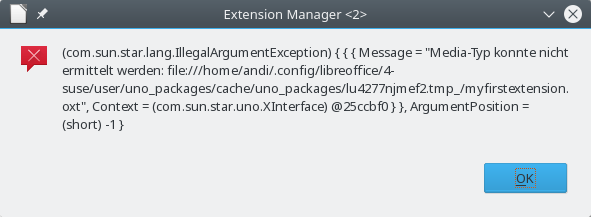
\includegraphics[width=0.7\linewidth]{pics/error_deinstallation_missing_manifest}
\captionof{figure}{Fehlermeldung wegen fehlender Datei manifest.xml beim Entfernen der Extension}
\label{fig:error_deinstallation_missing_manifest}
\end{center}

Wir legen dazu ein Unterverzeichnis \glqq META-INF\grqq~und in diesem eine neue Datei manifest.xml an. Die Datei bekommt zunächst nur folgenden Inhalt:
\begin{lstlisting}
<?xml version="1.0" encoding="UTF-8"?>
<manifest:manifest 
    xmlns:manifest="http://openoffice.org/2001/manifest">
</manifest:manifest>
\end{lstlisting}

Zu den möglichen weiteren Inhalten dieser Datei wird an späterer Stelle  in diesem Dokument Näheres erläutert.



\section{Erstellen der Extension-Datei}

Mit diesen ersten Versionen der Dateien description.xml und manfest.xml können wir nun eine Testversion der Extension-Datei erstellen und versuchen, die Extension noch ohne Funktionalität mit dem Extensionmanager zu installieren (und wieder zu deinstallieren)
Bei der Extension-Datei (*.oxt) handelt es sich um einen komprimierten Container. Um diesen zu erstellen, können Sie dem für die Test-Extension erstellten folgendes Python-Buildskript hinzufügen. Dieses Skript hat Björn Michaelsen erstellt. Es steht unter der Mozilla Public License (MPL) und ist beispielsweise hier zu finden:\linebreak \url{https://gerrit.libreoffice.org/gitweb?p=sdk-examples.git;a=blob;f=BundesGit/build;h=4e29b2addb081599100c5e8b48c384bbfff427ca;hb=HEAD}

Das Skript setzt voraus, dass im Verzeichnis eine weitere Textdatei mit dem Namen extensionname.txt vorhanden ist, die den Namen der Extension enthält, hier den Text
\begin{lstlisting}
myfirstextension.oxt
\end{lstlisting}
Das Build-Skript mit dem Namen build sieht folgendermaßen aus:
\begin{lstlisting}
#!/usr/bin/env python
# This Source Code Form is subject to the terms of the 
# Mozilla Public License, v. 2.0. If a copy of the MPL was  
# not distributed with this file, You can obtain one at 
# http://mozilla.org/MPL/2.0/.

from zipfile import ZipFile
import os, os.path, sys
scriptdir = os.path.dirname(os.path.abspath(sys.argv[0]))
extensionname = open(
    os.path.join(scriptdir, 
        'extensionname.txt')).readlines()[0].rstrip('\n')
with ZipFile(extensionname, 'w') as tuesdayzip:
    os.chdir(scriptdir)
    for root, dirs, files in os.walk('.'):
        for name in files:
            if not name == extensionname:
                tuesdayzip.write(os.path.join(root, name)) 
\end{lstlisting}
Da das Skript in der Programm-Sprache Python geschrieben ist, müssen Sie darauf achten, dass die Einrückungen korrekt übernommen werden. Das Skript selbst rufen Sie später einfach mit
\begin{lstlisting}
python ./build
\end{lstlisting}
auf. Die Extension-Datei wird dadurch in dem Verzeichnis der Test-Extension erstellt.

\section{Erste Testinstallation der Extension}

Die gerade erstellte OXT-Datei installieren wir nun testweise mit dem Extensionmanager von LibreOffice. Wir starten dazu LibreOffice und wählen im Menü Extras den Eintrag "Extension Manager". In der sich öffnenden Dialogbox aktivieren wir die Schaltfläche "Hinzufügen" und navigieren in dem nun geöffneten Datei-Dialog zu der gerade erstellten OXT-Datei und bestätigen die Auswahl über die Schaltfläche "Öffnen". Die neue Extension sollte anschließend im Dialogfenster gelistet sein.
\begin{center}
	\captionsetup{type=figure}
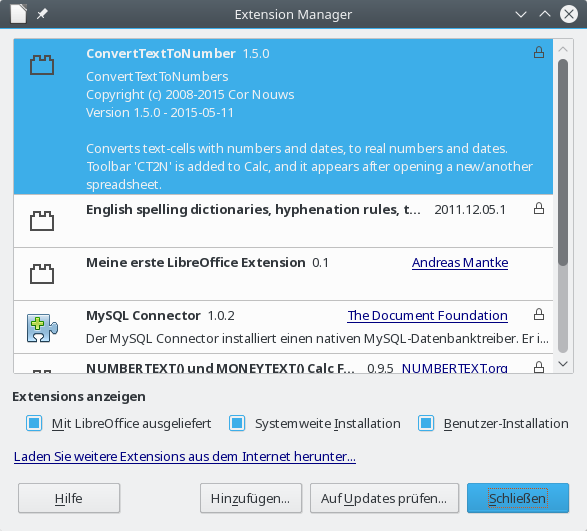
\includegraphics[width=0.7\linewidth]{pics/extensionmanager_extension_load01}
\captionof{figure}{Der LibreOffice Extension Manager nach Installation der neuen Extension}
\label{fig:extensionmanager_extension_load01}
\end{center}



Auf der rechten Seite des Eintrags für die neue Extension befindet sich der Name des Autors verbunden mit einem Link zu der URL, die in dem <name>-Tag innerhalb des <publisher>-Tags angegeben wurde. Dieser kann mit einem Mausklick im Standard-Browser aufgerufen werden.

Markieren Sie nun den neuen Eintrag im LibreOffice Extension Manager und deinstallieren Sie die Extension wieder über die nun angezeigte Schaltfläche "Entfernen". Die Extension sollte sich damit nach Bestätigen des folgenden Benutzerdialogs fehlerfrei entfernen lassen. Sofern dies nicht der Fall ist, könnte dies beispielsweise an einer fehlenden Datei manifest.xml (siehe dazu oben).

\section{Weitere Einträge in der Datei description.xml}

Auf der Abbildung im letzten Abschnitt ist zu sehen, dass für die Test-Extension im LibreOffice Extension Manager keine Grafik bzw. ein Logo angezeigt wird, wie beispielsweise für den MySQL Connector. Um ein solches Logo einzubinden, existiert der <icon>-Tag.

Erstellen Sie nun ein neues Unterverzeichnis \glqq images \grqq und anschließend eine neue Grafik bzw. ein neues Logo im Dateiformat PNG und der Dimension 42 mal 42 Pixel. Die Grafikdatei speichern Sie dann unter dem Namen \verb|"extensionicon_42.png"| im neuen Unterverzeichnis. Um das Logo einzubinden, fügen Sie dem <description>-Tag folgenden Eintrag hinzu:

\begin{lstlisting}
<icon>
    <default xlink:href="images/extensionicon_42.png" />
</icon>
\end{lstlisting}

In dem Tag hinter \glqq xlink:href \grqq wird die relative URL zu der Grafikdatei angegeben. Neben dem Link zu der Default-Grafik ist es möglich, parallel eine alternative Grafik mit hohem Kontrast, mit einem weiteren Tag anzugeben:
\begin{lstlisting}
<high-contrast xlink:href="(...)" />
\end{lstlisting}

\paragraph*{Minimale LibreOffice Version}$~~$\\

Es ist möglich, für die Extension eine minimale Version von LibreOffice anzugeben. Dies geschieht über den <dependencies>-Tag. Dieser Tag braucht eine Namespace-Deklaration, die hinter \glqq xmlns:lo \grqq erfolgt. Innerhalb der <dependencies>-Tag wird dann mit einem weiteren Tag die minimale LibreOffice-Version, für das Beispiel Version 4.2.

\begin{lstlisting}
<dependencies xmlns:lo=
    "http://libreoffice.org/extensions/description/2011">
    
    <lo:LibreOffice-minimal-version name="LibreOffice 4.2" 
        value="4.2"/>
    
</dependencies>
\end{lstlisting}

Die Vorgabe einer auch maximalen Version von LibreOffice, wie dies früher für OpenOffice.org möglich war, steht nicht mehr zur Verfügung. Der Tag für die Angabe der minimalen LibreOffice-Version erfordert neben der Übergabe des Wertes (\glqq value \grqq ) mit der Nummer des Releases (nur zweistellig, nicht ein etwaiges Micro-Release) auch die Vorgabe des Namens als Zeichenkette. Für die Anzeige der Meldung über die minimal erforderliche LibreOffice-Version im Extension Manager wird allerdings nur auf das angegebene Value zurückgegriffen.

\paragraph*{Beschreibung der Extension}$~~$\\

Der Extension kann eine Erläuterung Ihrer Funktionsweise über den <extension-description>-Tag hinzugefügt werden, wobei dieser mehrere Lokalisierungen dieser Beschreibung aufzunehmen.

Hierzu legen wir zunächst ein weiteres Unterverzeichnis \glqq description \grqq und darin zwei neue -zunächst leere Textdateien \verb|"description_de.txt"| und \verb|"description_en.txt"| an. Diese können später mit Informationen in deutscher und englischer Sprache befüllt werden. Wir binden diese beiden Beschreibungsdateien über folgende Ergänzung des <description>-Tag ein:
\begin{lstlisting}
<extension-description>
    <src xlink:href="description/description_en.txt" 
        lang="en" />
    <src xlink:href="description/description_de.txt" 
        lang="de" />
</extension-descritption>
\end{lstlisting}

Der in ihnen abgelegte Text wird nach der Installation im Extension Manager als Erläuterung angezeigt. Er sollte daher möglichst kurz und präzise formuliert werden und gegebenenfalls für ausführlichere Informationen auf eine externe Ressource (z.B. eine Webseite oder ein Wiki) verweisen.

Die Bezeichner für die Lokalisierung richten sich nach \href{https://tools.ietf.org/html/rfc3066}{RFC 3066}. Es sind daher sowohl Lokalisierungsbezeichner in der zuvor benutzten Form als auch spezifischere zulässig wie beispielsweise:
\begin{lstlisting}
<src (...) lang="en-GB" />
<src (...) lang="en-US" />
\end{lstlisting}

\paragraph*{Release Notes}$~~$\\

Es ist zwar möglich, in der Datei description.xml ein Tag für Release-Notes vorzugeben, allerdings hat dies für den Anwender keinen praktischen Nutzen, da ihm die Verbindung zu einer in dem <release-notes>-Tag eingestellten Verbindung zu einer URL im Extension Manager nicht angezeigt wird. Sofern für den Anwender wichtige Informationen zur Funktionsweise der Extension und zu Änderungen des oder der Release angezeigt werden sollten, eignet sich daher allein der zuvor beschriebene <description>-Tag und eine darin verlinkte externe Ressource am besten.

\paragraph*{Registration / Lizenz}$~~$\\

Das Registration-Element ermöglicht im Moment allein die Vorgabe der Lizenz der Extension, wobei auch hier wieder die Möglichkeit der parallelen Übermittlung von unterschiedlichen Lokalisierungen besteht.

Das <registration>-Element enthält ein <simple-license>-Element, welches wieder für jede Lokalisierung ein <license-text>-Element enthält. Das <simple-license>-Element enthält ein notwendiges Attribut \glqq accept-by \grqq . Optional sind zwei weitere Attribute in diesem Element möglich: \glqq suppress-on-update\grqq~ und \glqq suppress-if-required\grqq .\\

\begin{tabular}{|p{3.5cm}|p{8.3cm}|}
	\hline \rowcolor{hellgrau} \rule[-3ex]{0pt}{5.5ex}  Attribut & Beschreibung \\
	\hline \rule[-3ex]{0pt}{5.5ex} accept-by & Erforderlich. Der Wert kann entweder \glqq user\grqq~ oder \glqq admin\grqq~ sein. \glqq user\grqq~ bedeutet, dass jeder Benutzer der Lizenz zuzustimmen hat. Dies heißt dann, dass die Extension nur vom Benutzer und nicht vom Administrator als systemweite (shared) Extension installiert werden kann. Sofern der Wert \glqq admin\grqq~ gesetzt ist, kann die Extension auch als shared (geteilt / systemweit) installiert werden. In diesem Fall muss lediglich die Person, die die Extension installiert, der Lizenz zustimmen. Die einzelnen Benutzer werden nicht gefragt, ob sie die Lizenz akzeptieren. Sie können die Extension einfach benutzen.\\
	\hline \rule[-3ex]{0pt}{5.5ex}	suppress-on-update & Optional. Falls das Attribut nicht gesetzt ist, wird als Wert \glqq false\grqq~ angenommen. Sofern das Attribut mit dem Wert \glqq true\grqq~ vorgegeben ist, wird bei einem Update der Extension (gleiche ID, aber eventuell andere Version) der Lizenzdialog nicht erneut angezeigt.\\
	\hline \rule[-3ex]{0pt}{5.5ex}	suppress-if-required & Optional. Falls das Attribut nicht gesetzt ist, wird als Wert \glqq false\grqq~ angenommen. Der Wert \glqq true\grqq~ weist darauf hin, dass der Lizenzdialog während der Installation nicht angezeigt wird, sofern dies gewünscht wird. Dies kann dann durch den Schalter  \verb|--suppress-license| von unopkg vorgegeben werden und wird implizit für mitgelieferte (gebündelte) Extensions vorausgesetzt.\\
	\bottomrule
	
\end{tabular}

\bigskip
\bigskip
Legen Sie nun ein weiteres Unterverzeichnis \glqq registration\grqq~ und darin die Textdateien \verb|"license_de.txt"| und \verb|"license_en.txt"| an. Es reicht zunächst, wenn die Dateien existieren, auch wenn sie aktuell noch keinen Inhalt haben. Ihr späterer Inhalt wird, sofern nicht in der Einstellung unterdrückt, dem Benutzer im Installationsdialog angezeigt. In dem Dialog wird dann abgefragt, ob er die Lizenz akzeptiert.

\begin{lstlisting}
<registration>
    <simple-license accept-by="admin">
        <license-text xlink:href="registration/license_de.txt" 
            lang="de" />
        <license-text xlink:href="registration/license_en.txt" 
            lang="en" />
    </simple-license>
</registration>
\end{lstlisting}

Die Datei description.xml hat mit den weiteren vorgenommenen Ergänzungen nun folgenden Inhalt:

\begin{lstlisting}
<?xml version="1.0" encoding="UTF-8"?>
<description
    xmlns="http://openoffice.org/extensions/description/2006"
    xmlns:xlink="http://www.w3.org/1999/xlink">

    <identifier value="org.mycompany.myfirstextension" />
    <version value="0.1" />
    <platform value="all" />
    <display-name>
        <name lang="de">
            Meine erste LibreOffice Extension</name>
        <name lang="en">
            My first LibreOffice extension</name>
    </display-name>
    <publisher>
        <name xlink:href="http://amantke.de/blog">
            Andreas Mantke</name>
    </publisher>
    <icon>
        <default xlink:href="images/extensionicon_42.png" />
    </icon>
    <dependencies xmlns:lo=
        "http://libreoffice.org/extensions/description/2011">
        <lo:LibreOffice-minimal-version name="LibreOffice 4.2" 
            value="4.2"/>
    </dependencies>
    <extension-description>
        <src xlink:href="description/description_en.txt" 
            lang="en" />
        <src xlink:href="description/description_de.txt" 
            lang="de" />
    </extension-description>
    <registration>
        <simple-license accept-by="admin">
            <license-text 
                xlink:href="registration/license_de.txt" 
                lang="de" />
            <license-text xlink:href="registration/license_en.txt" 
                lang="en" />
        </simple-license>
    </registration>
</description>

\end{lstlisting}

Eine entsprechende Basisvorlage für eine LibreOffice Extension finden Sie im Github-Repository unter folgender Adresse:
\url{https://github.com/andreasma/extensionbook/tree/master/extensiontemplates/extension_basic_design/example01}.

\chapter{Auslieferung von Inhalten mit Extensions}

MIt einer LibreOffice Extension lassen sich verschiedene Arten von Inhalten dem Standard-Programm hinzufügen. So ist es beispielsweise möglich, der Gallery, einem Verwaltungsmodul für Grafiken, Zeichnungen, Musik und andere Multimediadateien, neue Bereiche und Dateien hinzuzufügen. Wie Sie eine solche Extension erstellen, soll im folgenden Abschnitt erläutert werden.

\section{Gallery-Extension}

Bevor wir eine Gallery-Extension erstellen können, müssen wir zunächst mit LibreOffice ein entsprechendes neues Gallery-Thema erstellen, das wir dann mit neuen Inhalten (z.B. Grafiken) befüllen und die entstandenen Dateien exportieren.

\subsection{Neues Gallery-Thema erstellen}

Beginnen wir also mit dem Erstellen eines neuen Gallery-Themas in LibreOffice. Starten Sie das Programm. Die Gallery rufen Sie über das Menü \glqq Ansicht\grqq~und den dortigen Eintrag \glqq Gallery\grqq~auf. Die Gallery wird damit in der Seitenleiste geöffnet (früher wurde sie oberhalb des Bearbeitungsfensters unterhalb der Menüleiste angezeigt). Im oberen Bereich werden die vorhandenen Themen in Ihrem LibreOffice angezeigt Erstellen Sie nun über die Schaltfläche \glqq Neues Thema\grqq~und den folgenden Dialog ein solches Thema. Auf dem ersten Register (\glqq Allgemein\grqq) des Dialogs geben Sie einen Namen für das Thema vor. Sofern Sie bereits zuvor Grafiken, Zeichnungen oder Multimedia-Dateien erstellt haben, können Sie diese über das Register \glqq Dateien\grqq~direkt dem Thema hinzufügen. Wir nennen das Thema \glqq Tiere\grqq~, da wir einige Grafiken mit offenen Lizenzen aus dem Openclipart-Projekt in unserer Beispiel-Extension in der LibreOffice-Gallery verfügbar machen wollen.

\begin{center}
	\captionsetup{type=figure}
	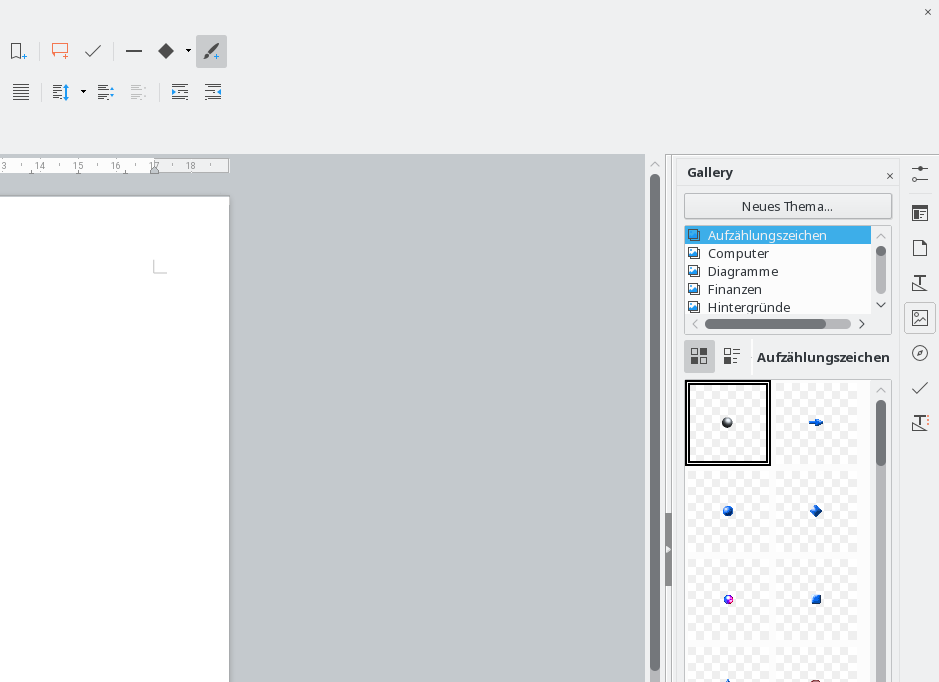
\includegraphics[width=0.9\linewidth]{pics/libreoffice_gallery}
	\captionof{figure}{Die LibreOffice Gallery}
	\label{fig:libreoffice_gallery}
\end{center}


Die Grafiken auf der Seite von OpenClipart (https://openclipart.org) werden dort unter Public Domain veröffentlicht. Dort wird dazu die Creative Commons Zero 1.0 Public Domain License (https://creativecommons.org/publicdomain/zero/1.0/) verwendet.

Für unser gerade erstelltes Tier-Thema  in der Gallery laden wir mehrere Tiergrafiken von der OpenClipart-Webseite möglichst im Vektorformat (SVG) herunter, z.B. einen Elefanten (Elephant), einen Tiger und einen Wolf. Wir können diese Grafiken nun im SVG-Dateiformat in das gerade erstellte Thema der Gallery einfügen. Dazu rufen wir mit einem rechten Mausklick auf das Thema das Kontextmenü auf und dort wählen dort den Eintrag \glqq Eigenschaften\grqq~aus. Damit gelangen wir wieder in den Dialog, in dem wir auf dem Register \glqq Dateien\grqq~neue Grafiken oder andere Dateien dem Thema hinzufügen können. Oben im Dialog können wir in dem Ausklappmenü hinter Dateitypus vorgeben, welche Art von Datei wir hinzufügen wollen. Nach einem Mausklick auf die Schaltfläche \glqq Hinzufügen\grqq~ öffnet sich der Dateidialog, mit dem wir zu dem Verzeichnis und der Datei navigieren, die wir einfügen wollen. Über die Schaltfläche \glqq Öffnen\grqq~ wird das Hinzufügen sodann ausgelöst.

Zwar ist es möglich, SVG-Grafiken in die Gallery einzufügen, allerdings führt dies aktuell regelmäßig dazu, dass LibreOffice längere Zeit für das Hinzufügen benötigt, sehr viel Systemressourcen (CPU-Power) beansprucht und sich später auch beim Einfügen von Grafiken aus der Gallery in ein Dokument sehr viel Zeit nimmt bzw. scheitert. Die Grafiken sollten daher zunächst in ein Pixel-Dateiformat wie beispielsweise PNG umgewandelt werden. Dafür kann z.B. das Programm Inkscape (https://inkscape.org/de/) verwandt werden, sofern eine Umwandlung nicht auf der Kommandozeile erledigt werden soll.

\begin{center}
	\captionsetup{type=figure}
	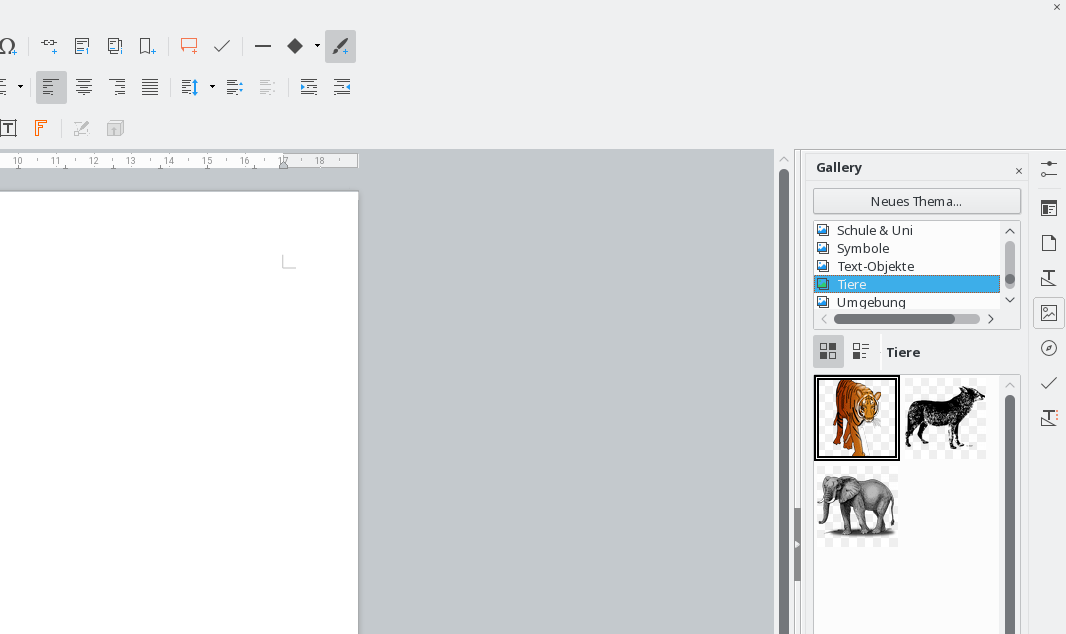
\includegraphics[width=0.9\linewidth]{pics/libreoffice_gallery_new_theme_with_graphics}
	\captionof{figure}{Das neue Gallery-Thema mit einigen Grafiken}
	\label{fig:libreoffice_gallery_new_theme_with_graphics}
\end{center}


\bigskip\textbf{Exkurs}
\\

Auf der Kommandozeile lassen sich Grafiken mit dem Programm \glqq convert\grqq~aus dem Programmpaket ImageMagick konvertieren. Soll nur von einem Dateiformat in ein anderes konvertiert werden, reicht ein einfaches Kommando nach folgendem Muster:
\begin{lstlisting}
convert datei1.svg datei1.png
\end{lstlisting}

Die Datei \glqq datei1.svg\grqq~wird damit in die das Dateiformat PNG umgewandelt. Das Programm convert bietet darüber hinaus aber sehr viele Möglichkeiten, Grafiken schnell und komfortabel auf der Kommandozeile und viele Dateien in einem Durchgang zu bearbeiten.
Ein Überblick zu den vielfältigen Optionen lässt sich auf der Seite https://www.imagemagick.org/script/convert.php gewinnen. Das Programmpaket ImageMagick ist sowohl für das Linux Betriebssystem und andere Betriebssysteme der Nix-Welt als auch für das Betriebssystem Windows verfügbar. Es kann von der Projektseite (https://www.imagemagick.org) heruntergeladen oder beispielsweise unter dem Betriebssystem Linux als Paket der jeweiligen Distribution installiert werden.

\subsection{Die Dateien des neuen Gallery-Themas}

Das neue Gallery-Thema ist nun erstellt und einige Dateien eingefügt worden. Es wurde von LibreOffice unter den Konfigurationsdateien des Benutzers abgelegt. Der genaue Speicherort und der Dateiname wird angezeigt, wenn im Kontextmenü des neuen Gallery-Themas der Befehl \glqq Eigenschaften\grqq~aufgerufen wird. Auf dem Register \glqq Allgemein\grqq~wird hinter \glqq Ort\grqq~der Pfad und Name des neuen Themas angezeigt. Ein Gallery-Thema besteht immer aus drei Dateien mit den Dateiendungen \glqq sdg\grqq, \glqq sdv\grqq~und \glqq thm\grqq. LibreOffice vergibt für ein neues Thema aktuell immer Dateinamen mit der Zeichenkette \glqq neues thema\grqq. Die Dateinamen lassen sich ändern. Es ist allerdings darauf zu achten, dass alle drei zusammengehörenden Dateien eines neuen Themas den gleichen Dateinamen vor der Dateiextension erhalten. Wir benennen die Dateien des neuen Themas also um in \glqq tiere.sdg\grqq, \glqq tiere.sdv\grqq~und \glqq tiere.thm\grqq. Damit haben wir die Gallery-Dateien für die neue Beispiel-Gallery-Extension fertig gestellt und können damit die Extension erstellen.

\subsection{Bauen der Gallery-Extension}

Im Kapitel \nameref{oxtcontainerinhalt} haben wir ein erste LibreOffice Extension in Ihrer Grundstruktur erstellt. Diese Extension soll nun um die weitere Funktionalität einer Gallery-Extension erweitert werden. Dazu legen wir im Grundverzeichnis einen weiteren Ordner \glqq gallery\grqq~ an und kopieren in diesen die vorhergehenden Abschnitt erstellten drei Gallery-Dateien. Im Grundverzeichnis erstellen wir weiterhin eine neue Textdatei \glqq paths.xcu\grqq.

\bigskip\textbf{Die Datei paths.xcu}
\\

Die Datei paths.xcu beginnt mit einer XML-Definition, gefolgt von einer XML-Struktur:

\begin{lstlisting}
<?xml version="1.0" encoding="UTF-8"?>

<oor:component-data oor:name="Paths" 
    oor:package="org.openoffice.Office" 
    xmlns:install="http://openoffice.org/2004/installation" 
    xmlns:oor="http://openoffice.org/2001/registry"
    xmlns:xs="http://www.w3.org/2001/XMLSchema" 
    xmlns:xsi="http://www.w3.org/2001/XMLSchema-instance">
    
    <node oor:name="Paths">
        <node oor:name="Gallery" oor:op="fuse">
    	    <node oor:name="InternalPaths">
    	        <node oor:name="%origin%/gallery" 
    	            oor:op="fuse"/>
    	    </node>
    	</node>
    </node>
    
</oor:component-data>
\end{lstlisting}

Zunächst wird ein XML-Element für eine Extension definiert, die keinen Programmcode enthält. Darauf folgt der Pfad, in dem der Inhalt abgelegt werden soll. Mit dem Schlüsselwort \glqq InternalPaths\grqq~werden alle Verzeichnisse gekennzeichnet, die etwas enthalten können, die der Benutzer nicht ändern, aber beispielsweise durch Extension-Pakete erweitern, also mit eigenen Inhalten bevölkern kann. Hier ist es die LibreOffice Gallery. Das Schlüsselwort \glqq fuse\grqq~bewirkt das Vereinigen von bisherigem Inhalt der Gallery mit neuem Inhalt. Sofern bereits ein Verzeichnis mit dem entsprechenden Namen vorhanden ist, wird der Inhalt der Extension hinzugefügt, andernfalls wird ein neues Verzeichnis mit dem entsprechenden Namen angelegt.

Wenn Sie die Datei paths.xcu mit dem zuvor dargestellten Inhalt erstellt haben, wird diese allerdings noch nicht in der Extension aktiv eingebunden. Dafür ist eine kleine Ergänzung in der in Kapitel \ref{oxtcontainerinhalt} erstellten Datei \glqq manifest.xml\grqq~um folgende Zeile erforderlich:
\begin{lstlisting}
<manifest:file-entry manifest:media-type=
"application/vnd.sun.star.configuration-data"  
manifest:full-path ="paths.xcu"/>
\end{lstlisting}  
Diese Zeile ist zwischen:
\begin{lstlisting}
<manifest:manifest 
    xmlns:manifest="http://openoffice.org/2001/manifest">
\end{lstlisting}

und

\begin{lstlisting}
</manifest:manifest>
\end{lstlisting}
einzufügen. Anschließend kann die LibreOffice Extension mit dem in Kapitel \ref{oxtcontainerinhalt} erstellten Buildskript gebündelt werden. Nach einer Installation der Extension mit dem LibreOffice Extension Manager sollte danach in der Gallery ein neues Thema \glqq Tiere\grqq~mit den entsprechenden Grafiken angezeigt werden.

Während der Installation werden Sie feststellen, dass Sie lediglich eine weiße Seite im Dialog \glqq Lizenzvertrag für die Extension-Software\grqq~angezeigt bekommen. Dies beruht darauf, dass die im Kapitel \ref{oxtcontainerinhalt} erstellten Dateien für die Lizenzinformationen noch ohne Inhalt sind. Bevor Sie eine Extension veröffentlichen müssen Sie diese Dateien bearbeiten und dort die erforderlichen Informationen ablegen.

Eine entsprechende Vorlage für eine LibreOffice Gallery Extension finden Sie im Github-Repository unter folgender Adresse:
\url{https://github.com/andreasma/extensionbook/tree/master/extensiontemplates/gallery_extension/galleryextensionexample01}.

\section{Template-Extension}

Mit einer LibreOffice Extension lassen sich den Anwendern auch Vorlagen (Templates) für ihre täglichen Arbeiten oder bestimmte Aufgaben zur Verfügung stellen. Die Vorlagen werden dann, sofern sie für einzelne Benutzer installiert werden, in seinem Benutzerprofil abgelegt. Wo sich diese Einstellungen und insbesondere die Vorlagen befinden (oder später befinden werden, sofern bisher noch keine vorhanden sind), erfahren Sie bei einem Aufruf von \glqq Optionen\grqq~im Menü \glqq Extras\grqq. Dort befindet sich unter \glqq LibreOffice\grqq~der Eintrag \glqq Pfade\grqq. Wenn Sie diesen auswählen, sehen Sie auf der rechten Seite im Dialog die einzelnen Pfade (Paths), so auch den für die Vorlagen (\glqq Dokumentvorlagen\grqq).

Gegenüber der Gallery-Extension aus dem vorhergehenden Abschnitt ändern sich für  eine LibreOffice Extension mit Dokumentvorlagen nur das Verzeichnis, in dem die Vorlagen abgelegt werden, und wenige Einträge in der Datei \glqq paths.xcu\grqq. Sofern der Eintrag zu den Pfaden für die Vorlagen in der Benutzerkonfiguration auf ein Verzeichnis \glqq templates\grqq~zeigt, ist lediglich das Wort \glqq gallery\grqq~durch das Wort \glqq template\grqq~zu ersetzen. Die Datei paths.xcu sieht dann wie folgt aus:

\begin{lstlisting}
<?xml version="1.0" encoding="UTF-8"?>

<oor:component-data oor:name="Paths" 
    oor:package="org.openoffice.Office" 
    xmlns:install="http://openoffice.org/2004/installation" 
    xmlns:oor="http://openoffice.org/2001/registry"
    xmlns:xs="http://www.w3.org/2001/XMLSchema" 
    xmlns:xsi="http://www.w3.org/2001/XMLSchema-instance">

    <node oor:name="Paths">
        <node oor:name="Template" oor:op="fuse">
            <node oor:name="InternalPaths">
                <node oor:name="%origin%/template" 
                    oor:op="fuse"/>
                </node>
            </node>
        </node>

</oor:component-data>
\end{lstlisting}
Nun fehlt noch das Verzeichnis mit den Dokumentenvorlagen. Dazu legen wir ein solches mit dem Namen \glqq template\grqq~im Grundverzeichnis an. Je nachdem welche Arten von Vorlagen mit der Extension zur Verfügung gestellt werden sollen, ist im Unterverzeichnis template sinnvoller Weise eine weitere Struktur mit eigenen Unterverzeichnissen anzulegen. Diese in der Dateihierarchie tieferen Unterverzeichnisse enthalten dann Dokumentenvorlagen zu einzelnen Themengebieten, beispielsweise Vorlagen für das Schreibprogramm Writer oder Präsentationsvorlagen.

Es gibt bereits einige von LibreOffice für die von ihm mitgelieferten Dokumentenvorlagen verwendete Unterverzeichnisnamen, die bei der Benennung der Unterverzeichnisse im Verzeichnis template der Extension berücksichtigt werden sollten. Sie können sich diese Struktur im Programmverzeichnis von LibreOffice im Unterverzeichnis /share/template/common ansehen. Einige Beispiele:
\begin{itemize}
	\item officore = Geschäftliche Korrespondenz
	\item offimisc = Sonstige geschäftliche Dokumente
	\item personal = Private Korrespondenz und Dokumente
	\item presnt = Präsentationsvorlagen
	\item layout = Präsentationshintergründe
	\item misc = Diverses
\end{itemize}

Um die Beispiel-Extension für Dokumentenvorlagen mit entsprechenden Dokumenten zu bevölkern, laden Sie von der LibreOffice Template-Seite htts://extensions.libreoffice.org/templates Vorlagendokumente aus verschiedenen Themenbereichen herunter, beispielsweise eine oder mehrere Briefvorlagen, Präsentationsvorlagen und Vorlagen für Lebensläufe.

Sie können auch weitere Unterverzeichnisse für themenspezifische Vorlagen anlegen, beispielsweise \glqq education\grqq~für Bildung oder \glqq magazine\grqq~für Zeitschriften- bzw. Magazin-Vorlagen. Entsprechende Vorlagendokumente finden Sie auf der LibreOffice Template Webseite.

Sofern Sie Ihre Beispiel-Vorlagen-Extension mit solchen weiteren Unterverzeichnissen mit entsprechenden Dokumentvorlagen ausgestattet haben, können Sie diese Themenbereiche in der Vorlagenverwaltung von LibreOffice gefiltert anzeigen lassen. Diesen Dialog rufen Sie über das Menü \glqq Datei - Vorlagen - Vorlagen verwalten\grqq~auf. Im Dialog können Sie dann filtern nach der Art der Dokumente, z.B. Textdokument, und nach Kategorien, z.B. Education. Sofern entsprechende Vorlagen vorhanden sind, werden Sie unten im Dialog angezeigt.

\begin{center}
	\captionsetup{type=figure}
	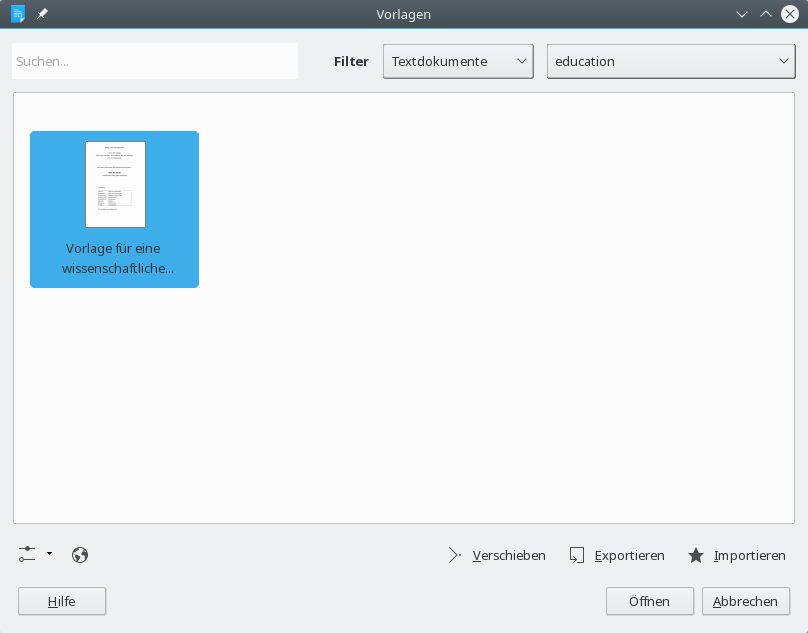
\includegraphics[width=0.9\linewidth]{pics/template_administration_dialog_with_new_template_section}
	\captionof{figure}{Der Dialog Vorlagen verwalten mit neuer Kategorie education}
	\label{fig:template_administration_dialog_with_new_template_section}
\end{center}



Die Benennung der Kategorie mit \glqq education\grqq~im Filter der Vorlagenverwaltung lässt sich wie auch die Benennung anderer Kategorien sprachlich anpassen. Dazu legen Sie im Verzeichnis \glqq template\grqq~der Extension eine neue Datei \glqq groupuinames.xml\grqq~an. Mit dieser werden dann für die einzelnen Kategorien die Namen gesetzt. Die Datei kann dann beispielsweise folgenden Inhalt bekommen:

\begin{lstlisting}[language={[LaTeX]TeX},inputencoding={utf8},extendedchars=false, escapeinside=``]
<?xml version="1.0" encoding="UTF-8"?>
<groupuinames:template-group-list
    xmlns:groupuinames=
        "http://openoffice.org/2006/groupuinames">
    <groupuinames:template-group groupuinames:name="education"
        groupuinames:default-ui-name="Bildung" />
    <groupuinames:template-group groupuinames:name="presnt"
        groupuinames:default-ui-name="Pr`ä`sentationen" />
</groupuinames:template-group-list>

\end{lstlisting}

Es ist nicht nötig, Verzeichnisnamen für Verzeichnisse aus der Standardinstallation von LibreOffice in der neuen XML-Datei erneut vorzugeben. Der zweite goupuinames-Eintrag war daher nicht erforderlich. Es wäre aber möglich gewesen, den mit der Extension neu im Unterverzeichnis \glqq presnt\grqq~verfügbar gemachten Präsentationsvorlagen einen abweichenden Kategorienamen zuzuordnen, beispielsweise \glqq Community-Präsentationen\grqq. Die von LibreOffice mitgelieferten Präsentationsvorlagen würden dann weiterhin mit der Kategorie \glqq Präsentationen\grqq~angezeigt, während die neuen der Extension unter \glqq Community-Präsentationen\grqq~eingeordnet wären.

Eventuell wollen Sie eine Extension mit Vorlagen für unterschiedliche Sprachen bauen, wobei dem Anwender nur die Vorlagen aufgelistet werden, die zu seiner Spracheinstellung passen. Dies ist mit den Einstellungen für eine Multilanguage-Template- bzw. Mehrsprachen-Vorlagen-Extension möglich. Zunächst werden im Unterverzeichnis \glqq template\grqq~für die vorgesehenen Lokalisierungen neue Unterverzeichnisse angelegt. Die Benennung hat dabei der ISO-Sprachkodierung zu folgen, also  beispielsweise \glqq en-US\grqq~für englischsprachige, \glqq de\grqq~für deutschsprachige und \glqq fr\grqq~für französischsprachige Vorlagen. In diesen Unterverzeichnissen für die einzelnen Lokalen, werden dann jeweils wieder Unterverzeichnisse für die einzelnen Kategorien angelegt. Um deren Darstellung bzw. Benennung im Kategorien-Filter des Vorlagenverwaltungs-Dialogs zu steuern, werden in den Unterverzeichnissen der Lokalen jeweils wieder \glqq groupuinames.xml\grqq~Dateien nach dem zuvor dargestellten Muster angelegt.

Danach bedarf es noch einer kleinen Änderung in der Datei \glqq paths.xcu\grqq. Dort ist die Zeile:
\begin{lstlisting}
<node oor:name="%origin%/template" oor:op="fuse"/>
\end{lstlisting}

durch die Zeile:
\begin{lstlisting}
<node oor:name="%origin%/template/$(vlang)" oor:op="fuse"/>
\end{lstlisting}

zu ersetzen. Die Ergänzung \glqq \$(vlang)\grqq~bewirkt, dass nur auf die Vorlagen der Extension in dem zur Spracheinstellung der Programmoberfläche passenden Unterverzeichnis zugegriffen und diese dem Anwender präsentiert werden. Die Vorlagen aus den Unterverzeichnissen mit anderen Sprachkodierungen werden ausgeblendet.

Es ist nicht möglich in der Extension zusätzlich noch einen Bereich mit sprachunabhängigen Vorlagen anzulegen. Sofern solche Vorlagen - beispielsweise Präsentationshintergründe - allen Benutzern, unabhängig von der Oberflächen-Spracheinstellung verfügbar sein sollen, ist ihre Ablage folglich in dem entsprechenden Unterverzeichnis jeder Lokale vorzunehmen.

\section{AutoText-Extension}

Das Erstellen von Textdokumenten lässt sich insbesondere auch im beruflichen Umfeld mit dem Aufruf von Textbausteinen deutlich beschleunigen und erleichtern. LibreOffice bietet dazu die Möglichkeit, sogenannte Autotexte zu speichern. Dies sind im Regelfall häufiger verwendete Texte, die in LibreOffice auch mit Grafiken, Tabellen und Feldbefehlen verbunden sein können. Mit solchen Autotexten lassen sich dann beispielsweise große Teile von Schriftsätzen erstellen und diese auch mit individualisierten Daten wie Aktenzeichen oder Datum des Bezugsschreibens versehen.

Im beruflichen Umfeld werden oft eine Vielzahl von Standardtexten entwickelt, mit denen sich Anfragen von Kunden und Lieferanten schnell, effektiv und zielgenau beantworten lassen. Solche Standardtexte können, nachdem sie von einem Anwender erstellt worden sind, mit Hilfe einer Extension verteilt und so allen Benutzern zugänglich gemacht werden.

Erster Schritt auf dem Weg zu einer AutoText-Extension ist das Erstellen von Autotexten. Diese werden dann von LibreOffice in einem gezippten Archiv mit der Dateiendung \glqq bau\grqq~im Benutzerverzeichnis gespeichert. Wo dieses für den Benutzer abgelegt wird, erfahren Sie bei Aufruf von \glqq Optionen\grqq~im Menü Extras von LibreOffice in dem Dialog unter \glqq LibreOffice - Pfade\grqq. Dort ist der Pfad (oder mehrere) hinter dem Eintrag \glqq AutoText\grqq~gelistet.

Welche Textbausteine in der installierten Version von LibreOffice für den Benutzer bereits vorhanden sind, lässt sich folgendermaßen prüfen:
\begin{itemize}
	\item Rufen Sie im Menü Extras den Befehl \glqq Makros - Makro ausführen\grqq~auf.
	\item Öffnen Sie im Dialog links \glqq LibreOffice Makros\grqq und unter diesen \glqq Gimmicks\grqq~sowie danach \glqq AutoText\grqq.
	\item Im Dialog auf der rechten Seite wählen Sie mit einem Mausklick \glqq Main\grqq.
	\item Schließen Sie den Dialog über die Schaltfläche \glqq Ausführen\grqq~ ab.
	\item Nach Ausführen des Makros wird Ihnen ein neues Dokument mit den verfügbaren Textbausteinen angezeigt, das Sie sich ausdrucken oder speichern können.
\end{itemize}

\begin{center}
	\captionsetup{type=figure}
	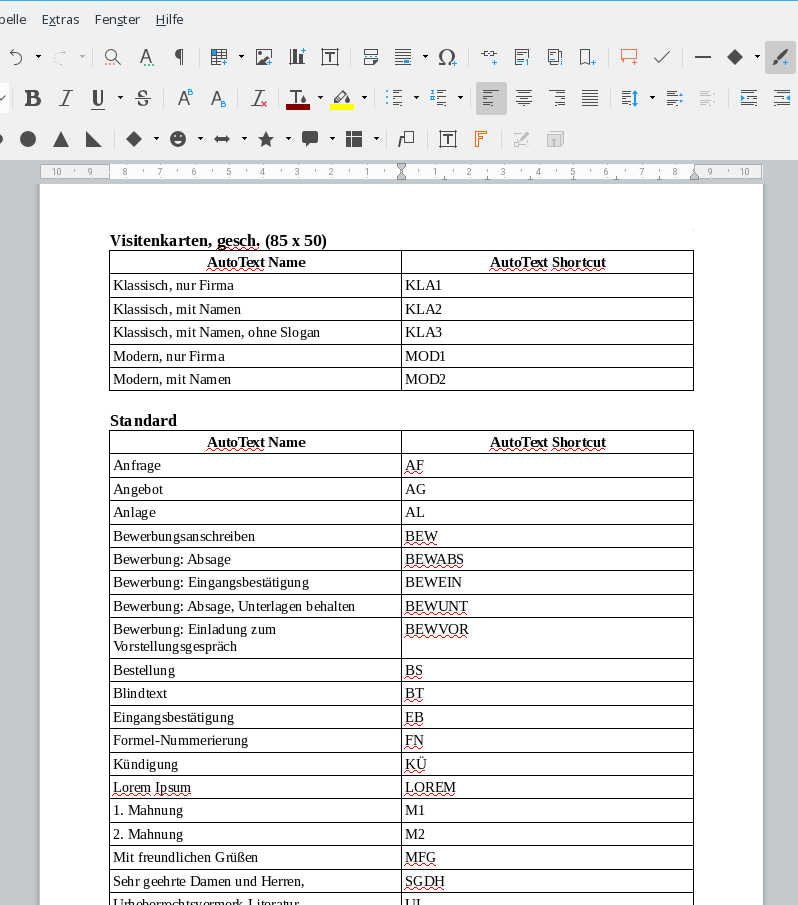
\includegraphics[width=0.9\linewidth]{pics/available_autotext}
	\captionof{figure}{Anzeige der verfügbaren Textbausteine}
	\label{fig:available_autotext}
\end{center}

Auch wenn auf dem System Autotexte in anderen Sprachen vorhanden sind, werden mit dem Makro nur diejenigen ausgegeben, die der Spracheinstellung der Oberfläche von LibreOffice entsprechen. Diese werden sortiert nach unterschiedlichen Kategorien aufgelistet, beispielsweise solche für Visitenkarten und solche für normale Textdokumente. Am Ende der Liste befindet sich ein Bereich bzw. eine Kategorie, in der Ihre eigenen Autotexte aufgelistet werden.

Nachdem Sie nun ermittelt bzw. angezeigt haben, welche Textbausteine bereits in Ihrem System vorhanden sind, geht es nun darum, neue Bausteine für eine AutoText-Extension zu erstellen. Dazu rufen wir in LibreOffice im Menü \glqq Extras\grqq~den Eintrag \glqq AutoText\grqq~auf. In dem aufgerufenen Dialog klicken Sie auf die Schaltfläche \glqq Pfad\grqq~und schauen Sie, ob der Pfad zum AutoText-Verzeichnis in den Konfigurations-Einstellungen Ihres Benutzers bereits existiert. Sofern er nicht existiert, fügen Sie diesen nun hinzu und schließen den Dialog über die Schaltfläche \glqq OK\grqq~ab. Danach rufen Sie im AutoText-Dialog die Kategorien über die entsprechende Schaltfläche auf. Fügen Sie dort oben im Feld \glqq Kategorie\grqq~den Namen Ihrer neuen Kategorie ein, z.B. \glqq Standardantworten\grqq. Unter Pfad wählen Sie den zuvor unter Pfaden eventuell hinzugefügten Pfad zu den Autotexten für Ihren Benutzer und schließen den Dialog über die Schaltfläche \glqq OK\grqq~ab. Sie haben damit im Unterverzeichnis \glqq autotext\grqq~eine neue gezippte bau-Datei mit dem Namen Ihrer Kategorie, also beispielsweise \glqq Standardantworten.bau\grqq.

Schließen Sie den AutoText-Dialog wieder und schreiben Sie Ihren ersten Textbaustein in das geöffnete Textdokument. Diesen Text markieren Sie danach und rufen wieder den AutoText-Dialog auf. Geben Sie im Feld Name nun die gewünschte Bezeichnung für Ihren Textbaustein und rechts ein Kürzel ein. Danach ordnen Sie den neuen Textbaustein noch einer Kategorie zu. Dazu wählen Sie die von Ihnen zuvor erstellte Kategorie im Feld unten aus. Danach klicken Sie auf die Schaltfläche \glqq AutoText\grqq~und wählen im Ausklappmenü \glqq Neu\grqq~aus. Damit haben Sie Ihren Textbaustein der Kategorie hinzugefügt. Nach Schließen des AutoText-Dialogs verfahren Sie entsprechend mit weiteren Textbausteinen, die Sie für die neue Extension verfassen wollen. Die AutoTexte sind dann jeweils unter Eingabe des vorgegebenen Kürzels und die Taste \glqq F3\grqq~einzufügen.

Nachdem Sie nun die Bau-Dateien mit den Textbausteinen fertig gestellt haben, müssen diese nur noch in eine LibreOffice extension eingebaut werden. Sie erstellen dazu zunächst ein Unterverzeichnis \glqq autotext\grqq~im Grundverzeichnis der Extension. Danach erstellen Sie eine neue oder bearbeiten Sie die Datei \glqq paths.xcu\grqq, die sich ebenfalls im Extension-Grundverzeichnis befinden muss. Die Datei sollte danach folgenden Inhalt haben:


\begin{lstlisting}
<?xml version="1.0" encoding="UTF-8"?>

<oor:component-data oor:name="Paths" 
    oor:package="org.openoffice.Office" 
    xmlns:install="http://openoffice.org/2004/installation" 
    xmlns:oor="http://openoffice.org/2001/registry"
    xmlns:xs="http://www.w3.org/2001/XMLSchema" 
    xmlns:xsi="http://www.w3.org/2001/XMLSchema-instance">

    <node oor:name="Paths">
        <node oor:name="AutoText" oor:op="fuse">
            <node oor:name="InternalPaths">
                <node oor:name="%origin%/autotext" 
                    oor:op="fuse"/>
            </node>
        </node>
    </node>
</oor:component-data>
\end{lstlisting}

Gegenüber der im vorhergehenden Abschnitt erläuterten Vorlagen-Extension ändern sich in der Autotext-Extension das Schlüsselwort Name. Dieses lautet nunmehr \glqq AutoText\grqq. Außerdem ändert sich natürlich auch der Pfad zu dem Verzeichnis, in dem die Textbaustein-Zip-Dateien liegen. Dieser verweist auf das Unterverzeichnis \glqq autotext\grqq. In letzteres Unterverzeichnis kopieren Sie nun die von Ihnen erstellten Textbaustein-Zip-Dateien. Danach bauen Sie die Extension mit dem Python-Build-Skript. Entfernen Sie aus dem Autotext-Verzeichnis ihrer Benutzerkonfiguration die erstellten Textbaustein-Zip-Archive und kontrollieren Sie, dass Ihre Textbausteine sich nicht mehr in der Liste der Autotexte befinden. Im Anschluss installieren sie mit dem Extension-Manager ihre AutoText-Extension. Sie sollten nun wieder ihre Textbausteine in der Liste der Autotexte angeboten bekommen.

Die Textbausteine werden regelmäßig nur für eine Spracheinstellung von LibreOffice sinnvoll verwendbar sein, so dass die Autotexte nach Lokalisierungen gruppiert im Unterverzeichnis \glqq autotext\grqq~abgelegt werden sollten. Dazu erstellen Sie für jede Lokalisierung, für die Sie eine Textbaustein-Zip-Datei generiert haben, ein Unterverzeichnis, dessen Benennung der ISO-Sprachkodierung folgt, also  beispielsweise \glqq en-US\grqq~für englischsprachige, \glqq de\grqq~für deutschsprachige und \glqq fr\grqq~für französischsprachige Vorlagen. Die angelegten Unterverzeichnisse dürfen später nicht leer sein, d.h., sie müssen jeweils zumindest eine Textbaustein-Zip-Datei enthalten. Andernfalls wird nach der Installation der Extension bei einem Zugriff auf das Verzeichnis im Rahmen des Aufrufs der AutoText-Funktion eine Fehlermeldung angezeigt.

Sofern Sie die Textbausteine nach Lokalisierungen gruppiert in Unterverzeichnissen ablegen, müssen Sie die Datei \glqq paths.xcu\grqq~anpassen. Dort ist die Zeile:
\begin{lstlisting}
<node oor:name="%origin%/autotext" oor:op="fuse"/>
\end{lstlisting}

durch die Zeile:
\begin{lstlisting}
<node oor:name="%origin%/autotext/$(vlang)" oor:op="fuse"/>
\end{lstlisting}

zu ersetzen.

Eine entsprechende Vorlage für eine LibreOffice AutoText-Extension finden Sie im Github-Repository unter folgender Adresse:
\url{https://github.com/andreasma/extensionbook/tree/master/extensiontemplates/auto-text_extension/autotextextensionexample01}.

\section{Autokorrektur-Extension}

Eine weitere schöne Möglichkeit besteht darin, LibreOffice eigene automatische Korrekturen (Autokorrektur) beizubringen und diese anschließend in eine Extension verpackt an andere Benutzer auszuliefern. Diese Autokorrektur-Funktion hat einen Beitragenden zu LibreOffice dazu gebracht, eine Erweiterung namens PCSteno für LibreOffice zu erstellen. Diese besteht aus einer selbst erstellten Autokorrektur-Datei \verb|acor_de-DE.dat|, die vom Anwender in das Unterverzeichnis \glqq autocorr\grqq~kopiert werden muss. Nach einem Neustart von LibreOffice kann damit mit wenigen Tastaturanschlägen Text schnell eingegeben werden. Der Benutzer muss allerdings die entsprechenden Kürzel/Abkürzungen erlernen; z.B. \glqq nmh\grqq~ für \glqq nicht mehr\grqq~ oder \glqq svj\grqq~ für \glqq soviel\grqq.

Das Ganze lässt sich allerdings auch eleganter mit einer LibreOffice-Extension an den Anwender ausliefern. Wie dies funktioniert, soll nun kurz unter Verwenden des Beispiels PCSteno gezeigt werden. Zunächst muss ein neues Verzeichnis \glqq testpcsteno\grqq~ erstellt werden. Darin legen wir eine Datei \verb|descrciption.xml| etwa mit folgendem Inhalt an:

\begin{lstlisting}
<?xml version="1.0" encoding="UTF-8"?>
<description
    xmlns="http://openoffice.org/extensions/description/2006"
    xmlns:xlink="http://www.w3.org/1999/xlink">
    <identifier value="org.libreoffice.testpcsteno" />
    <version value="0.2" />
    <platform value="all" />
    <display-name>
        <name lang="de">Test PC Steno für Libreoffice</name>
        <name lang="en">Test PC Steno for LibreOffice</name>
    </display-name>
    <publisher>
        <name xlink:href="http://amantke.de/blog">
        Andreas Mantke</name>
    </publisher>
</description>
\end{lstlisting}

Für das Beispiel habe ich im Wert (value) des Identifiers \glqq libreoffice\grqq~ als Namen des Unternehmems eingesetzt und als Veröffentlicher (Publisher) meinen eigenen Namen und mein Blog eingetragen. Für die Veröffentlichung der entsprechenden Extension sind diese Werte durch die Daten des Extension-Autors zu ersetzen.

Damit die Extension auch deinstalliert werden kann, muss noch eine Datei \verb|manifest.xml| in einem Unterverzeichnis \verb|META-INF| hinzugefügt werden:
\begin{lstlisting}
<?xml version="1.0" encoding="UTF-8"?>
<manifest:manifest 
  xmlns:manifest="http://openoffice.org/2001/manifest">
    <manifest:file-entry
     manifest:media-type="application/
     vnd.sun.star.configuration-data" 
     manifest:full-path ="paths.xcu"/>
</manifest:manifest>
\end{lstlisting}

In dieser Datei wird eine Datei \verb|paths.xcu| referenziert, die nun noch zu erstellen ist mit folgendem Inhalt:

\begin{lstlisting}
<?xml version='1.0' encoding='UTF-8'?>

<oor:component-data 
    oor:package="org.openoffice.Office" 
    oor:name="Paths" 
    xmlns:install="http://openoffice.org/2004/installation" 
    xmlns:oor="http://openoffice.org/2001/registry" 
    xmlns:xs="http://www.w3.org/2001/XMLSchema" 
    xmlns:xsi="http://www.w3.org/2001/XMLSchema-instance">

    <node oor:name="Paths">
        <node oor:name="AutoCorrect" oor:op="fuse">
            <node oor:name="InternalPaths">
                <node oor:name="%origin%/autocorr" 
                  oor:op="fuse"/>
                </node>
            </node>
    </node>
</oor:component-data>
\end{lstlisting}

Nach den allgemeinen Definitionen werden in den Zeilen beginnend mit \glqq node\grqq~ die speziellen Daten für eine Autokorrektur-Extension gesetzt. Der oor:name wird mit \glqq AutoCorrect\grqq~ definiert und der Pfad wird auf das Verzeichnis \glqq autocorr\grqq~ gesetzt. Die übrigen Vorgaben in den Node-Tags entsprechen denen, die bereits weiter oben im Abschnitt zur Gallery-Extension besprochen wurden.

Nun fehlt noch die Autokorrektur-Datei, die mit der Extension verteilt werden soll. Dazu erstellt man ein neues Unterverzeichnis \verb|autocorr|. In dieses wird sodann die Datei \verb|arcor_de-DE.dat| abgelegt.

Die Extension kann nun mit dem Build-Skript, das oben im Abschnitt \glqq Erstellen der Extension-Datei\grqq~ beschrieben und erstellt wurde. Diese Datei \verb|build| mit dem enthaltenen Python-Skript muss sich ebenfalls im in diesem Abschnitt angelegten Verzeichnis \glqq testpcsteno\grqq~ befinden. Sein Aufruf ist ebenfalls oben beschrieben.

\begin{center}
	\captionsetup{type=figure}
	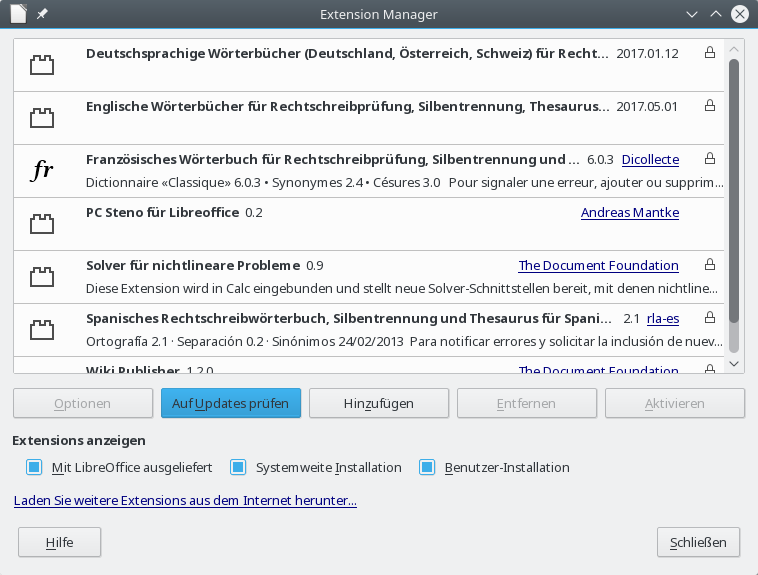
\includegraphics[width=0.9\linewidth]{pics/extensionmanager_autocorrect_extension_installed01}
	\captionof{figure}{Anzeige Autokorrektur-Extension im Extension-Manager nach Installation}
	\label{fig:autocorr_extension_extension_manager}
\end{center}



Es ist auch für Autokorrektur-Extensions möglich, die Autokorrekturen nach Lokalisierungen auszuliefern. Dazu ist die Zeile
\begin{lstlisting}
<node oor:name="%origin%/autocorr" oor:op="fuse"/>
\end{lstlisting}

durch
\begin{lstlisting}
<node oor:name="%origin%/autocorr/$(vlang)" oor:op="fuse"/>
\end{lstlisting}

zu ersetzen. In dem Unterverzeichnis ist für die auszuliefernden Lokalisierungen ein Unterverzeichnis anzulegen und die Autokorrektur-Datei dort abzulegen. Als Beispiel für die Lokalisierung Deutsch ist somit ein Unterverzeichnis \glqq de\grqq~ anzulegen und darin die Autokorrektur-Datei für diese Lokalisierung abzulegen.

Mit der Installation der Autokorrektur-Extension wird allerdings für LibreOffice eine zuvor vom Benutzer erstellte eigene Autokorrektur-Liste(/-Datei) nicht mehr sichtbar. Sie bleibt zwar im Unterordner \glqq autocorr\grqq~ erhalten, die dort enthaltenen Korrekturen sind allerdings für den Benutzer nicht mehr verfügbar. Sie gehen jedoch nicht komplett verloren, sondern sind nach der Deinstallation der Autokorrektur-Extension für den Benutzer wieder verfügbar. Die mit der Extension übermittelte Autokorrektur-Datei genießt somit Priorität vor der Datei im Unterverzeichnis \glqq autocorr\grqq.

Da sich bei der Einbindung von Extensions Änderungen ergeben haben, ist es wichtig, zumindest eine minimale Version von LibreOffice anzugeben. Da ältere Versionen von LibreOffice keine Sicherheitsupdates mehr erhalten, sollte als minimale Version zumindest LibreOffice 4.2 gewählt werden (mit dieser Version gab es einige Änderungen für Extensions). Der Datei \verb|description.xml| werden hierfür folgende Zeilen hinzugefügt:
\begin{lstlisting}
<dependencies xmlns:lo=
  "http://libreoffice.org/extensions/description/2011">
    <lo:LibreOffice-minimal-version name="LibreOffice 4.2" 
      value="4.2"/>
</dependencies>
\end{lstlisting}

Der Extension fehlt nun noch eine Beschreibung, die sowohl eine Erläuterung des Zwecks als auch der Funktionsweise der Extension gibt. Hierzu gibt es das Description-Tag, das auf eine entsprechende Textdatei mit der Beschreibung verweisen kann. Es ist dabei möglich, für jede Lokalisierung auf eine eigene Datei zu verweisen. Die hier als Beispiel gewählte Autokorrektur-Erweiterung PCSteno ist nur in deutscher Sprache lokalisiert. Es soll jedoch dennoch bereits die Lokale im Description-Tag vorgesehen werden. Die Ergänzung zur Datei \verb|description.xml| lautet dann folgendermaßen:
\begin{lstlisting}
<extension-description>
    <src xlink:href="description/description_de.txt" 
      lang="de" />
</extension-descritption>
\end{lstlisting}

Nun muss noch ein Unterverzeichnis \glqq description\grqq~ erstellt und dort eine neue Textdatei \verb|description_de.txt| angelegt werden. Diese Datei kann einen längeren Beschreibungstext enthalten, es ist allerdings nicht sinnvoll, dort eine vollständige Dokumentation unterzubringen, da das Rendern im Extension-Manager bei längeren Texten nicht optimal ist. Es sollten daher nur einige grundsätzliche Erläuterungen und Hinweise aufgenommen werden und im Übrigen auf eine Datei mit der vollständigen Dokumentation verwiesen werden, die beispielsweise auf der LibreOffice Extensions-Website \verb|http://extensions.libreoffice.org/extensions| vom Autor der Extension zum Download (im Dateiformat ODT oder PDF) bereit gestellt werden kann.

Bevor die Extension auf der LibreOffice Extensions-Website veröffentlicht werden kann, ist die Datei \verb|description.xml| noch um den Verweis auf die Lizenz zu ergänzen, unter der die Extension veröffentlicht wird und die vom Anwender bei der Installation akzeptiert werden muss. Hierzu wird zunächst ein weiteres Unterverzeichnis \glqq registration\grqq~ angelegt, in dem, gegebenenfalls in unterschiedlichen Lokalisierungen Dateien mit den Lizenztexten abgelegt werden, z.B. für die deutsche Lokalisierung \verb|license_de.txt|. 

Anschließend wird die Datei \verb|description.xml| um folgende Eintragung ergänzt:
\begin{lstlisting}
<registration>
    <simple-license accept-by="admin">
        <license-text xlink:href="registration/license_de.txt" 
          lang="de" />
    </simple-license>
</registration>
\end{lstlisting}

Unsere Beispiel-Autokorrektur-Extension ist zwar aktuell nur in deutscher Sprache lokalisiert, allerdings ist es immer sinnvoll, die Extension von Beginn an auf eine mögliche Lokalisierung in anderen Sprachen vorzubereiten.

Sofern in Bezug auf ein Release der Extension besondere Informationen zu geben sind, insbesondere wenn sich die Bedienung verändert oder weitere Funktionen hinzugekommen sind, können der Extension besondere Release-Notes hinzugefügt werden. Hierzu gibt es das entsprechende XML-Tag. Allerdings werden diese Release-Notes dem Anwender in LibreOffice selbst aktuell nicht angezeigt. Er kann sich diese nur ansehen, wenn er die Extension-Datei entpackt und dort die Release-Notes-Datei mit einem Anzeigeprogramm für Textdateien oder einem Texteditor öffnet. Insoweit sind entsprechende Beigaben der Extension für den Anwender nur etwas erschwert wahrzunehmen. Dies sollte den Autor einer Extension trotzdem nicht davon abhalten, entsprechende Release-Notes der Extension beizufügen.

Eine entsprechende Vorlage für eine LibreOffice Autokorrektur-Extension finden Sie im Github-Repository unter folgender Adresse:
\url{https://github.com/andreasma/extensionbook/tree/master/extensiontemplates/autocorrect_extension/autocorrectextensionexample01}.


\section{Farbpaletten-Extension}

LibreOffice bringt eine Reihe von Farb-Paletten mit. Sie können sich die verfügbaren Paletten beispielsweise in dem Dialog \glqq Fläche\grqq~anzeigen lassen, den Sie im Programmmodul Draw im Menü \glqq Format\grqq~aufrufen können.

\begin{center}
	\captionsetup{type=figure}
	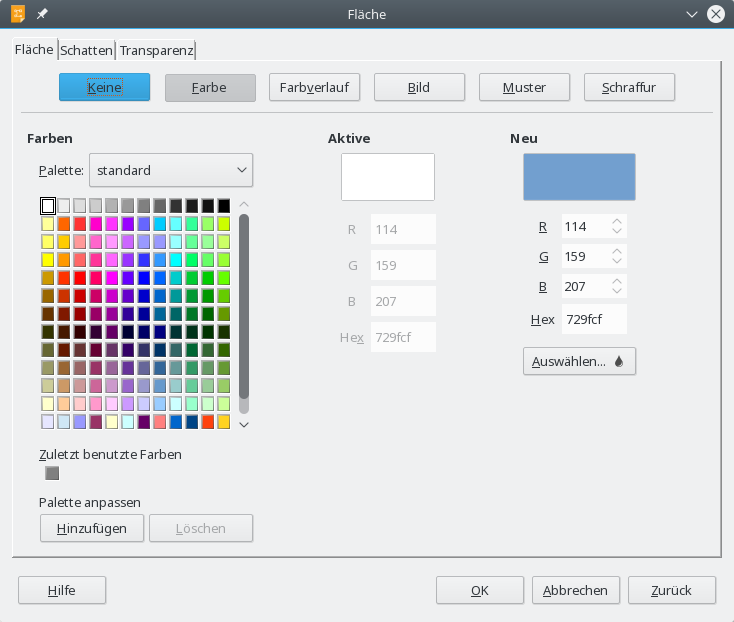
\includegraphics[width=0.9\linewidth]{pics/dialog_flaeche}
	\captionof{figure}{Der Dialog Fläche}
	\label{fig:dialog_flaeche}
\end{center}

Sie können nun eigene Farb-Paletten beispielsweise für spezielle Anwendungsfälle, etwa für die Corporate Identity eines Unternehmens, erstellen und anschließend mittels einer LibreOffice-Extension verteilen.

Zunächst erstellen Sie im Grundverzeichnis der Farbpaletten-Extension ein neues Unterverzeichnis \glqq palette\grqq. In diesem Unterverzeichnis erstellen Sie eine neue Datei mit dem Namen der Palette und der Dateiendung \glqq soc\grqq, zum Beispiel \glqq meinefirma.soc\grqq. Rufen Sie die neue Datei in einem Texteditor auf und fügen Sie Folgendes dort ein:

\begin{lstlisting}
<?xml version="1.0" encoding="UTF-8"?>
<!-- https://meinefirma.de -->
<ooo:color-table xmlns:office=
    "urn:oasis:names:tc:opendocument:xmlns:office:1.0"
    xmlns:draw="urn:oasis:names:tc:
      opendocument:xmlns:drawing:1.0"
    xmlns:xlink="http://www.w3.org/1999/xlink"
    xmlns:svg="http://www.w3.org/2000/svg"
    xmlns:ooo="http://openoffice.org/2004/office">
    
</ooo:color-table>
\end{lstlisting}

Innerhalb des XML-Tag <ooo:color-table> legen Sie danach die einzelnen Farben nach folgendem Muster and:

\begin{lstlisting}
<draw:color draw:name="Farbname" 
    draw:color="#Farbkodierung in Hexadezimal" />
\end{lstlisting}

Anstelle von Farbname tragen Sie dabei den individuellen Namen ihre benutzerdefinierten Farbe ein. Hinter \glqq draw color\grqq~ folgt nach dem \glqq \#\grqq~die Farbe in hexadezimaler Kodierung. Sofern Sie nur die Werte ihrer Farben nur im System RGB vorliegen haben, können Sie den Dialog \glqq Fläche\grqq~zum Umrechnen in das Hexadezimal-System verwenden. Geben Sie dazu auf der rechten Seite einfach die RGB-Werte ein und lesen Sie den Wert im Feld \glqq Hex\grqq~ab.

Wenn Sie die Datei mit der Farbpalette fertig gestellt haben, müssen Sie noch die Datei \glqq paths.xcu\grqq~im Grundverzeichnis neu anlegen oder ändern mit folgendem Inhalt:


\begin{lstlisting}
<?xml version="1.0" encoding="UTF-8"?>

<oor:component-data oor:name="Paths" 
    oor:package="org.openoffice.Office" 
    xmlns:install="http://openoffice.org/2004/installation" 
    xmlns:oor="http://openoffice.org/2001/registry"
    xmlns:xs="http://www.w3.org/2001/XMLSchema" 
    xmlns:xsi="http://www.w3.org/2001/XMLSchema-instance">

    <node oor:name="Paths">
        <node oor:name="Palette" oor:op="fuse">
            <node oor:name="InternalPaths">
                <node oor:name="%origin%/palette" 
                    oor:op="fuse"/>
            </node>
        </node>
    </node>
</oor:component-data>
\end{lstlisting}

Der Unterschied gegenüber den zuvor beschriebenen LibreOffice-Extensions besteht in der Bezeichnung hinter \glqq oor:name\grqq~, der nun \glqq Palette\grqq~lautet, sowie dem Pfad in dem weiteren Knoten, der nun auf das Unterverzeichnis \glqq palette\grqq~verweist.

Mit der nun fertig gestellten Datei \glqq paths.xcu\grqq~können Sie die Extension wieder mit dem in der Vorlage enthaltenen Skript \glqq build\grqq~automatisch bauen lassen.

Eine entsprechende Vorlage für eine LibreOffice Farbpaletten-Extension finden Sie im Github-Repository unter folgender Adresse:
\url{https://github.com/andreasma/extensionbook/tree/master/extensiontemplates/color_extension/colorextensionexample01}.


\chapter{Konfigurationseinstellungen mit einer Extension verteilen}

Mit Konfigurations-Extensions steht Ihnen die beste Methode bereit, um LibreOffice an die Arbeitsumgebung einer Organisation (z.B. eines Unternehmen oder einer Behörde) anzupassen und die entsprechenden Standardeinstellungen zu setzen. Dazu wird dann einfach die Konfigurations-Extension zusammen mit LibreOffice auf einem Computer installiert und alle Benutzer dieses Computers werden diese neuen Standardeinstellungen vorfinden und verwenden.

\end{document}
